\chapter{夸克质量}

夸克不是自然界的渐近态，因此它们的质量无法在实验中直接测量。它们通常在某类微扰方案（如 $\overline{\mathrm{MS}}$）中、并在某个标度 $\mu$ 下加以定义。其数值仍然是标准模型参数中已知程度最差的量之一。在本节中，我将讨论如何从格点数据提取它们。

一旦通过对格点数据的拟合确定了系数 $A_\pi$ 等，就可以通过对式~18.3 求逆从强子谱提取上夸克、下夸克和奇异夸克的质量。正如我之前提到的，当前的格点模拟忽略了同位旋破缺效应，因此我们只能确定 $m = (m_u + m_d)/2$ 与 $m_s$。我将首先讨论这些，然后简要提及重夸克质量 $m_c$ 和 $m_b$ 的提取。

在淬火近似下，估计 $m$ 最直接的方法是将 $M_\pi^2/X^2$ 外推到物理值。这里 $X$ 是一个有量纲的量，如 $f_\pi$、$M_\rho$、$M_N$ 或 $M_\Delta$，它不依赖于 $m_s$，并实际上设定了格点标度 $1/a$。在上述各量中，使用 $M_\rho$ 最具争议性，因为它通过强相互作用衰变且宽度很大（170~MeV）。另一方面，$M_\rho$ 的格点数据最容易获得，且信号良好。此外，在淬火近似下 $\rho$ 不衰变。因此，在 QQCD 中用 $M_\rho$ 而非其他某个量来设定 $a$，可能带来整体的标度不确定度。从不同量提取的 $1/a$ 的离散程度约为 $10\%$，这一淬火近似所固有的不确定度将被视为整体系统误差。类似地，可以通过外推比值 $M_s/X$ 来设定 $m_s$，其中 $M_s$ 是任何依赖于 $m_s$ 的态，如 $M_K$、$M_{K^*}$、$M_\phi$ 或任何含奇异夸克的重子。世界数据显示，$M_s$ 的不同选择会导致 $m_s$ 出现约 $20\%$ 的离散。值得注意的是，如果假定关系 $M_{PS}^2 = B_{PS} m_q$（LQCD 尚未验证其在 $[m, m_s]$ 的整个区间内成立），并用 $M_K$ 来固定 $m_s$，那么若 $m$ 用 $M_\pi^2$ 设定，比值 $m_s/m$ 必须为 25.9。

在完整理论中，$X$ 通过海夸克效应依赖于 $m_s$，类似地 $M_s$ 依赖于 $m$。因此，$m$、$a$ 和 $m_s$ 必须通过求解耦合方程组来固定。

强子谱的模拟已由世界各地许多合作组完成，关于强子质量作为夸克质量与格距之函数的数据大量存在。（几乎所有格点合作组都对这些计算作出了贡献 [183]，例如 APE、哥伦比亚大学、CP-PACS、费米实验室、GF11、HEMCGC、JLQCD、洛斯阿拉莫斯、SCRI、交错（staggered）、UKQCD 和伍珀塔尔大学等合作组。）在早期的分析中，不同费米子方案之间的夸克质量估计相差几乎两倍，而离散化误差与淬火误差的模式在任何单个合作组的工作中都不明显。通过汇集威尔逊、三叶草和交错费米子的全部世界数据，这一问题得到了澄清 [183,184]。基于最新、最高统计量和大格点数据的 $m$ 的最终图景，对三种费米子方案如图~\ref{fig:34} 所示。此图清楚地显示，在 $1/a \sim 2$~GeV 处约 $\sim 2$ 倍的差异，在外推到 $a = 0$ 后缩小到约 $15\%$，即大部分差异可归因于离散化误差。

$m_s$ 随 $a$ 的变化行为非常相似。基于对 1997 年世界数据 [185] 的分析，在标度 $\mu = 2$~GeV 下淬火结果的汇总（单位 MeV）如下：

\begin{table}[htbp]
\centering
\begin{tabular}{lccc}
\toprule
          & $m(M_\pi)$ & $m_s(M_K)$ & $m_s(M_\phi)$ \\
\midrule
威尔逊    & 4.1(1)     & 107(2)     & 139(11)       \\
TI 三叶草 & 3.8(1)     & 99(3)      & 117(8)        \\
交错      & 3.5(1)     & 91(2)      & 109(5)        \\
\bottomrule
\end{tabular}
\caption*{基于对 1997 年世界数据 [185] 的分析，威尔逊、蝌蚪图改进的三叶草（TI Clover）和交错费米子方案在标度 $\mu = 2$~GeV 下的轻夸克质量淬火估计（单位 MeV）。}
\label{tab:light-quark-masses}
\end{table}

这些估计是通过以下 Ansätze（假设）获得的。
\begin{itemize}
\item 手征拟合仅保留式~18.3 所示的最低阶项。
\item 用 $M_\pi^2/M_\rho$ 来固定 $m$。
\item 对 $m_s$ 给出两种选择的结果：$M_K^2/M_\rho$ 和 $M_\phi/M_\rho$。（使用 $M_{K^*}/M_\rho$ 得到的数值与使用 $M_\phi/M_\rho$ 得到的几乎相同。这意味着对于 $m_s(M_\phi)$ 的选择，也可以等价地用 $M_{K^*}$ 而非 $M_\rho$ 来设定标度。）
\item 由于采用了线性手征拟合，$m_s(M_K) \equiv 25.9\,m$。
\item 格点方案与 $\overline{\mathrm{MS}}$ 方案之间的匹配因子 $Z_m$ 是蝌蚪图改进的 1 圈结果。
\item 向 $a = 0$ 的外推采用最低阶离散化误差，即对威尔逊和三叶草为 $O(a)$ 与 $O(\alpha_s a)$，对交错为 $a^2$ 的二次式。
\end{itemize}

威尔逊、蝌蚪图改进的三叶草（TI Clover）和交错结果之间估计的最终差异约为 $15\%$，如图~\ref{fig:34} 所示。这可能源于被忽略的高阶离散化误差，和/或源于 $Z$ 的非微扰估计与 1 圈估计之间的差异。类似地，$m_s$ 随用于提取它的态（$M_K$ 对 $M_\phi$，或等价地 $M_{K^*}$）而出现的约 $20\%$ 变化，可能源于淬火近似，或部分是在外推中仅保留最低阶离散化修正所造成的假象。要将这些离散化误差与淬火误差区分开，需要具有近似物理值轻夸克的精确非淬火数据。

\begin{figure}[htbp]
\centering
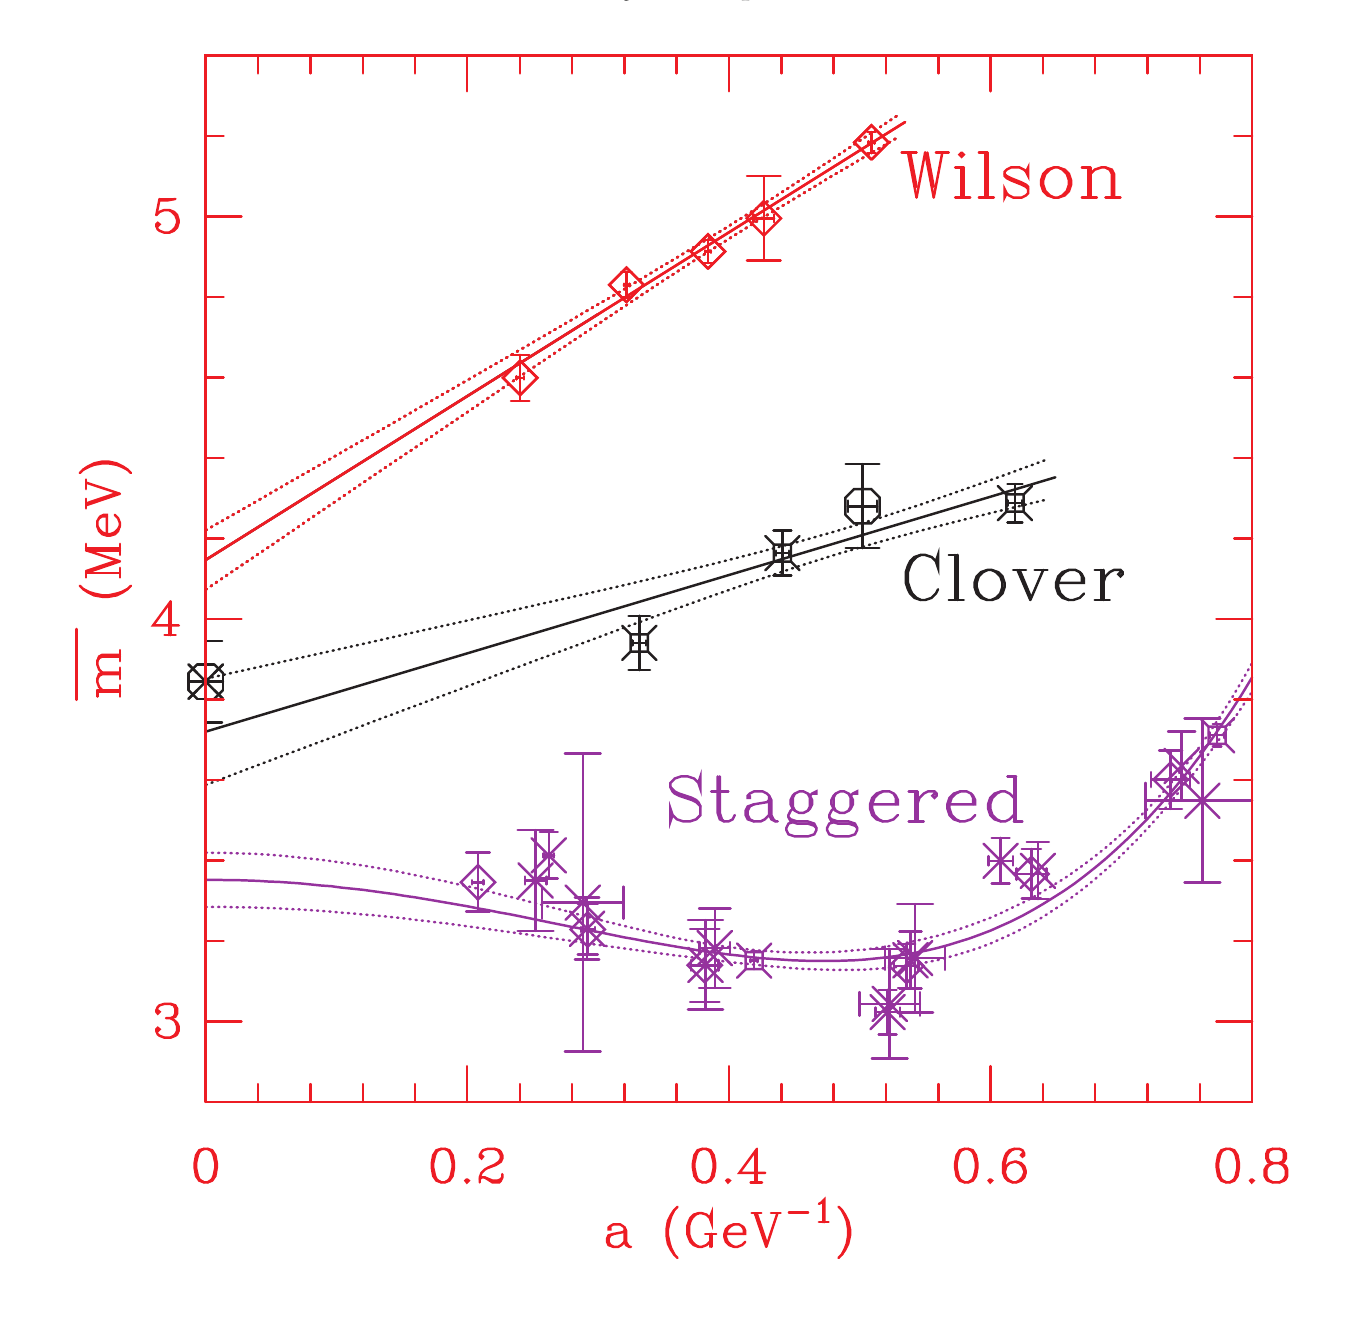
\includegraphics[width=0.8\textwidth]{images/fig34.png}
\caption{三种离散化方案——威尔逊、三叶草和交错——中 $m_u + m_d$ 随格距 $a$ 的变化行为。对威尔逊和三叶草方案显示了到 $a = 0$ 的线性外推，而对交错方案，拟合中同时包含了 $O(a^2)$ 和 $O(a^4)$ 项。三叶草方案中离散化误差的理论预期形式为 $O(\alpha_s a)$。用该形式外推得到的数值以 burst 符号标出。}
\label{fig:34}
\end{figure}

为了给出淬火结果的最佳估计，我对数据取平均，并把离散程度作为误差。在此基础上，我再加入一个因确定标度 $1/a$ 的不确定度而产生的 10\% 系统误差，该不确定度部分反映了淬火近似带来的不确定度。结果（在 $\overline{\mathrm{MS}}$ 方案中、在 2~GeV 处求值）为 [185]
\begin{equation}
\begin{aligned}
m &= 3.8(4)(4)~\mathrm{MeV}, \\
m_s &= 110(20)(11)~\mathrm{MeV}.
\end{aligned}
\end{equation}

\section{由沃德恒等式得到的轻夸克质量}

提取夸克质量的第二种方法基于轴矢流和矢量流的沃德恒等式
\begin{equation}
\begin{aligned}
Z_A\,\partial_\mu A_\mu &= (m_1 + m_2)_R\, Z_P\, P, \\
Z_V\,\partial_\mu V_\mu &= (m_1 - m_2)_R\, Z_S\, S,
\end{aligned}
\end{equation}
其中 1、2 是味指标，$P$ 和 $S$ 是格点赝标量与标量密度。由这些恒等式可以构造两点关联函数之比
\begin{equation}
\begin{aligned}
\frac{Z_P}{Z_A}\,\frac{\langle \partial_\mu A_\mu(\tau)\,P(0)\rangle}{\langle P(\tau)P(0)\rangle} &= (m_1 + m_2)_R, \\
\frac{Z_S}{Z_V}\,\frac{\langle \partial_\mu V_\mu(\tau)\,S(0)\rangle}{\langle S(\tau)S(0)\rangle} &= (m_1 - m_2)_R,
\end{aligned}
\end{equation}
一旦知道了各个重整化常数 $Z_i$，这些比值就给出重整化的夸克质量。由于沃德恒等式是算符恒等式，式~20.3 对所有 $\tau$ 都成立，只有在很短的时间上会受接触项的影响。因此，不需要像谱学方法中为分离最低态那样要求信号持续到渐近 $\tau$。

来自谱学和来自沃德恒等式的两种夸克质量估计，在连续极限下应当一致。对威尔逊作用量并使用 1 圈微扰 $Z$ 的两组数据的比较如图~\ref{fig:35} 所示。在有限 $a$ 处两种估计显著不同，然而线性外推对两组数据都适用，且外推值惊人地一致。因此可以把有限 $a$ 处的差异归因于离散化误差。

\begin{figure}[htbp]
\centering
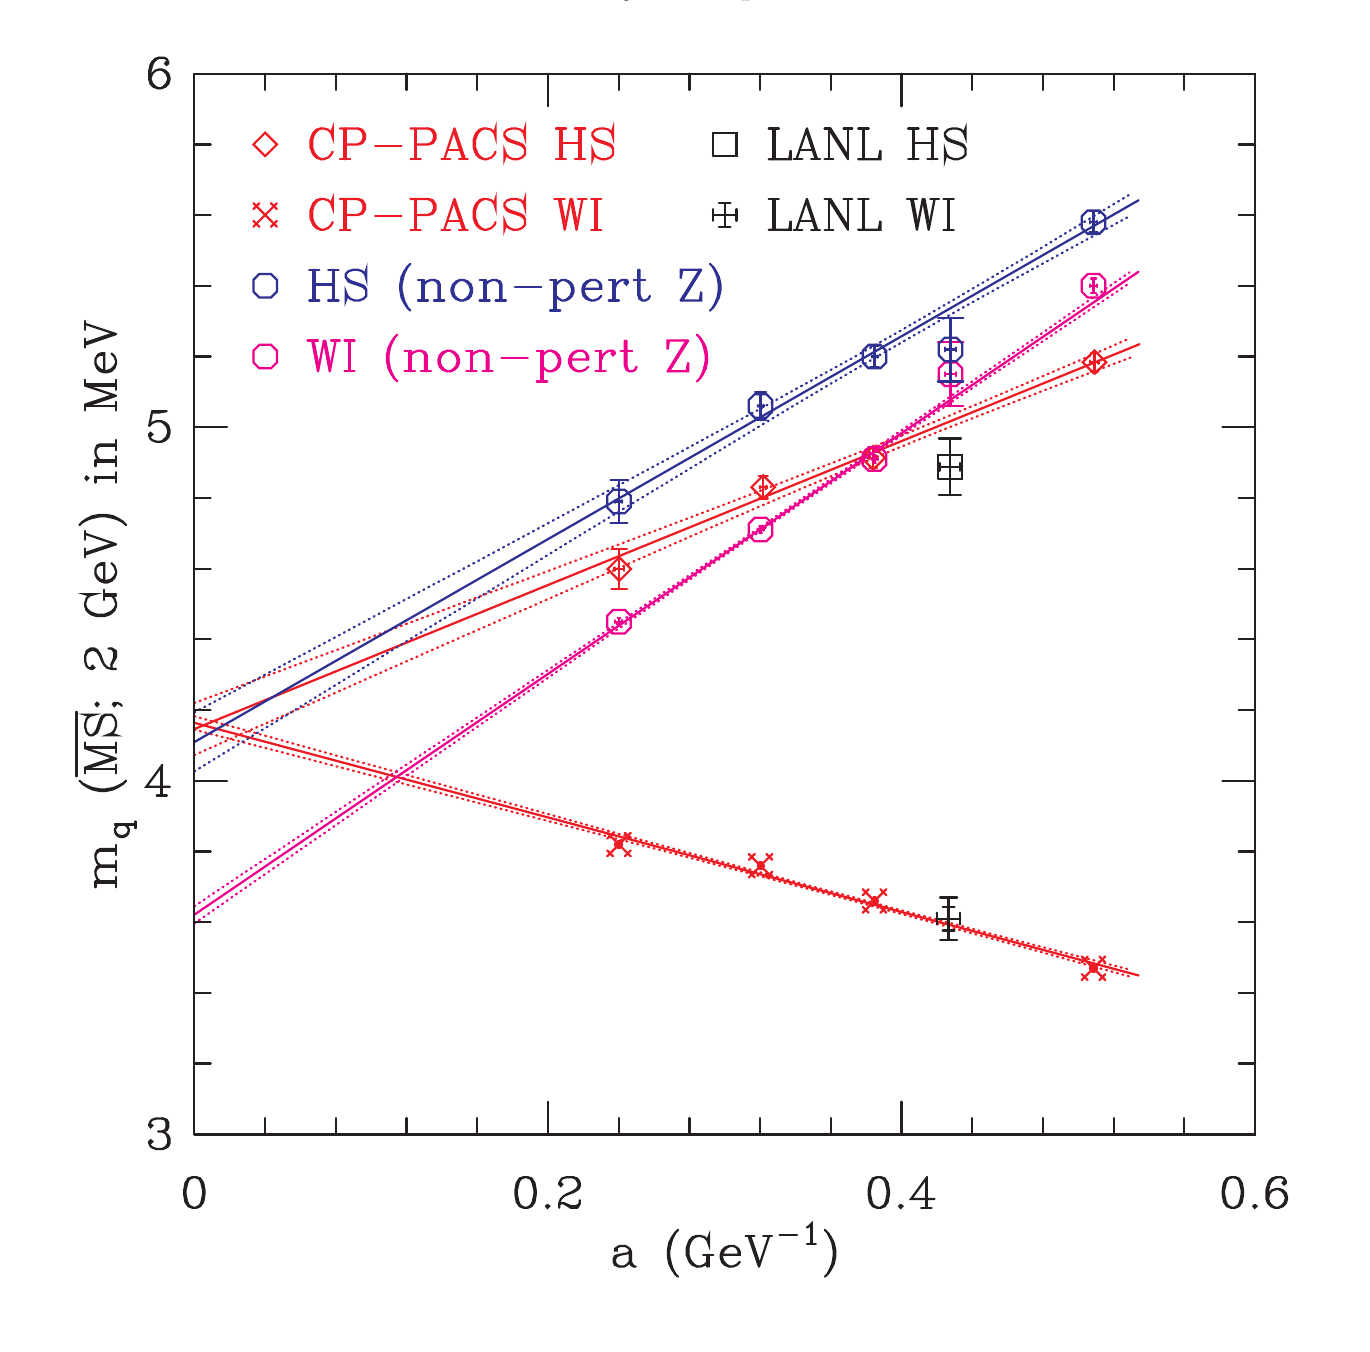
\includegraphics[width=0.8\textwidth]{images/fig35.png}
\caption{威尔逊费米子情形下 $m = (m_u + m_d)/2$ 随格距 $a$ 的变化行为。对两种估计重整化常数的方式——即 1 圈微扰与非微扰——分别显示了来自强子谱学方法和沃德恒等式方法的数据。}
\label{fig:35}
\end{figure}

最近对 $Z$ 的非微扰计算 [186] 对这一美好的图景提出了挑战。图~\ref{fig:35} 也显示了使用这些非微扰 $Z$ 分析同样的数据的结果。在固定 $a$ 处，非微扰 $Z$ 将强子谱学与 WI 两种结果都提高到大致相同的数值。这表明大部分差异源于对 1 圈 $Z$ 的 $O(\alpha_s^2)$ 修正，而非如前所述的 $O(a)$ 离散化误差。然而，$Z$ 的非微扰计算本身带有 $O(a)$ 误差，而这些误差在 [186] 的结果中尚未被分辨。因此，在这些 $Z$ 中，$O(a)$ 离散化误差与 $O(\alpha_s^2)$ 误差的效应无法被清晰地区分开。

底线是，尽管我们尚未分辨这两种误差，并且尽管在从 1 圈 $Z$ 换到非微扰 $Z$ 时，固定 $a$ 处的数值和随 $a$ 的斜率都显著增大，外推值却大致保持不变。

总而言之，我相信我们最终已经获得了轻夸克质量的数值，并对统计误差和除淬火之外的所有系统误差都有了可靠的估计。目前已在开展计算，显著增加 $n_f = 2$ 和 4 种动力学费米子味的数据点数量，以减小淬火不确定度。同时，非微扰计算重整化常数的新方法也正在发展之中。因此，我预期在未来几年内，QQCD 与完整 QCD 对轻夸克质量的估计精度都将显著提高。

\section{薛定谔泛函方法}

在上述讨论中，非微扰 $Z$ 一词仅指格点方案。在所需的匹配常数中，人们仍必须对连续方案中的重整化常数使用微扰表达式，并对匹配点做出良好的估计。ALPHA 合作组提出了一种方法，用以消除这最后一点对微扰论的依赖 [187]。他们方法的细节已由吕舍尔（Lüscher）教授在本学校讲解，因此我只概述要点。
\begin{enumerate}
\item[(i)] 在某个红外格点标度下，用轴矢 WI 方法计算夸克质量。同时在薛定谔泛函方案中非微扰地计算 $Z_P$ 和 $Z_A$。
\item[(ii)] 用非微扰计算的步进标度函数将这个格点结果演化到某个非常高的标度。
\item[(iii)] 在这个 $\alpha_s$ 很小的高标度下，定义与重整化群无关的质量
\begin{equation}
\hat{m} = \lim_{a\to 0} m_R \left[2\beta_0 g^2\right]^{-\gamma_0/2\beta_0}.
\end{equation}
\end{enumerate}
这个 $\hat{m}$ 与方案无关，因此后续在连续极限中、使用最精确版本（4 圈）的标度演化方程 [188]，即可在某种方案、某个所需标度下转换成流（running）质量。再次强调，这种方法的优点是格点计算直接预言标度与方案不变的量 $\hat{m}$。ALPHA 合作组的计算仍在进行中，目前尚未公布 $\hat{m}$ 的估计值。看看它们与上面讨论的常规强子谱学或 WI 方法相比如何，将会很有意思。我的看法是它们会非常相似。

\section{夸克质量在 CP 破坏中的作用}

轻夸克质量精确测定的一个非常适时的应用，是用标准模型预言由比值 $\epsilon'/\epsilon$ 表征的 K 介子衰变中的直接 CP 破坏（参见 Buras 教授的讲义及 [189]）。原因是 $\epsilon'/\epsilon$ 在很好的近似下正比于 $1/(m_d + m_s)^2$ [190]，
\begin{equation}
\epsilon'/\epsilon = A \left[c_0 + c_6 B_6^{3/2} + c_8 B_8^{3/2}\right] \left(\frac{158~\mathrm{MeV}}{m_s + m_d}\right)^2,
\end{equation}
其中所有量都应在标度 $m_c = 1.3$~GeV 处求值。式~20.5 突出显示了其对轻夸克质量和袋参数 $B_6^{3/2}$、$B_8^{3/2}$ 的依赖，后者也是预期由 LQCD 提供的。系数 $c_0$、$c_6$ 和 $c_8$ 已计算到次次领头阶，而随着 $M_{top}$ 现在已知，它们提取中的主要不确定度来自 $\Lambda_{QCD}$ 的值。在式~2.4 的参数化中，量 $A = |V_{ub}||V_{cb}| \sin\delta$ 需要输入其他标准模型参数，如 $f_B$、$|V_{ub}|$、$|V_{cb}|$、$B_K$、$B_{B_d} f_{B_d}$。使用 Buras 在标度 $m_c = 1.3$~GeV 处引用的中心值 [190]，可得到 $A = 1.29 \times 10^{-4}$、$c_0 = -1.4$、$c_6 = 7.9$、$c_8 = -4.0$。遗憾的是，这些量中的误差使最终的理论预言 $\epsilon'/\epsilon = 3.6(3.4) \times 10^{-4}$ [190] 非常不确定。

目前的实验估计为：来自费米实验室 E731 的 $7.4(5.9) \times 10^{-4}$ [191] 和来自欧洲核子研究中心 NA31 的 $23(7) \times 10^{-4}$ [192]。新一代实验——费米实验室 E832、欧洲核子研究中心 NA48 和 DA$\Phi$NE KLOE——将把不确定度减小到约 $1 \times 10^{-4}$。这些实验的首批结果（参见 L.~Fayard 的讲义）应可在未来几年内获得。因此，收紧理论预言非常重要。显然，LQCD 所给出的较低的夸克质量估计将显著增大直接 CP 破坏的幅度，并使其实验测定与验证变得容易得多。

\section{重夸克质量 $m_c$ 与 $m_b$}

重夸克 $m_c$ 和 $m_b$ 的质量已利用粲偶素与 Upsilon（底偶素）谱学计算得到。对重夸克存在两种不同的夸克质量定义——极点质量和 $\overline{\mathrm{MS}}$ 质量。极点质量定义为 $m^{(pole)} = (M_{onia} - E_{binding})/2$，其中 $M_{onia}$ 取自实验数据，$E_{binding}$ 在格点上计算。这一计算采用了两种途径，即 NRQCD [193] 和重夸克有效理论（HQET）[194]，且结果一致。$\overline{\mathrm{MS}}$ 质量的优点是免除了 $m^{(pole)}$ 所固有的重正化子（renormalon）歧义，它通过微扰论由 $m^{(pole)}$ 得到。目前的结果为
\begin{equation}
\begin{aligned}
m_b^{\overline{\mathrm{MS}}} &= 4.15(5)(20)~\mathrm{GeV} && \text{(APE)}, \\
m_b^{\overline{\mathrm{MS}}} &= 4.16(15)~\mathrm{GeV} && \text{(NRQCD)}.
\end{aligned}
\end{equation}
这些估计与其他非格点方法的测定一致。

对 $m_c^{\overline{\mathrm{MS}}}$ 的各种格点估计，一致性就不那么好了。目前的估计介于 $1.2 - 1.5$~GeV 之间。例如，APE 合作组 [195,186]、费米实验室合作组 [196,197] 以及 Bochkarev 和 Forcrand [198]（他们在格点上计算 QCD 求和规则中出现的关联函数）所研究的三种不同方法给出
\begin{equation}
\begin{aligned}
m_c^{\overline{\mathrm{MS}}} &= 1.525(40)(125)~\mathrm{GeV} && \text{(APE)}, \\
m_c^{\overline{\mathrm{MS}}} &= 1.33(8)~\mathrm{GeV} && \text{(Fermilab)}, \\
m_c^{\overline{\mathrm{MS}}} &= 1.22(5)~\mathrm{GeV} && \text{(B\&F)}.
\end{aligned}
\end{equation}
在现阶段，我不认为这一差异显著，因为并非所有计算中的各种系统误差都得到了同样好的解决。

\section*{小结与致谢}

我希望这些讲义能够成功地为格点QCD及数值数据分析提供教学式的介绍。毫无疑问，有些主题被遗漏了，许多内容只是概述。我的目的是给出一个广泛的概览。我着重提供基础知识，并通过强子谱、强耦合常数 $\alpha_s$ 和夸克质量的计算来说明蒙特卡洛数据的分析方法。Martinelli 教授除其他内容外，将讨论弱哈密顿量矩阵元的提取，而吕舍尔（Lüscher）教授将提供一个全景式的展望，说明未来的计算会是什么样子，以及借助更好的离散化方案可能实现的改进。我希望这些讲义合在一起，能提供足够的细节与令人兴奋的内容，激励你们中的一些人更深入地探索这一领域。

我向所有使这次 Les Houches 学校活动愉快而精彩的组织者、学生和工作人员表示感谢。对我而言，这无疑是一段难忘的六周时光。在准备这些讲义的过程中，我要感谢 G.~Bali、U.~Heller、C.~Michael、M.~Peardon 以及 CP-PACS 合作组，特别是 S.~Hashimoto 和 T.~Yoshie 提供了未发表的数据。特别感谢我的合作者 T.~Bhattacharya、D.~Daniel、G.~Kilcup、A.~Patel 和 S.~Sharpe，多年来我从他们那里学到了很多。最后，我要感谢 T.~Bhattacharya、D.~Daniel、W.~Lee 和 S.~Sharpe 校阅了这些讲义并提出建议。
